\documentclass[a4paper, 10pt]{article}
\usepackage{graphicx}   % Including figure files
\oddsidemargin=0cm
\evensidemargin=0cm
\topmargin=-1.2cm
\textwidth=17cm
\textheight=25cm
\pagestyle{empty}

\begin{document}

\section*{0. Co-Is}
Chris Morrison\\
Gigi Guzzo\\

\section*{1. title}

VISTA-VIPERS: Is cosmic shear in tension with Planck?

\section*{2. abstract}

First cosmic shear results from the ESO Kilo Degree Survey (KiDS) on the VST show a $\sim2.5\sigma$ tension in the cosmological parameter $S_8 \equiv \sigma_8 (\Omega_m/0.3)^{0.5}$ with respect to results from the Planck CMB satellite. Such a low amplitude $S_8$ was already hinted at in several previous cosmic shear surveys but the new KiDS results are arguably the most robust in terms of statistical precision as well as systematic error control. The dominant source of systematic error is the calibration of photometric redshifts. Inclusion of data from the overlapping VIKING survey on VISTA can significantly improve the redshift errors, but requires VST+VIKING images of deep spectroscopic survey regions for calibration. Whereas the VST is targeting these fields already, not all deep spectroscopic fields that are useful for this calibration are available in the VIRCAM archive: in particular the wide+deep VIPERS survey, which contains some 90,000 redshifts, is not covered. VISTA 5-band imaging on the VIPERS region will furthermore have significant legacy value, particularly for measuring stellar masses of the VIPERS galaxies.
 
\section*{7 A Scientific rationale}

Our cosmological model, $\Lambda$CDM, is sufficiently strange that, despite its great success describing the Universe we observe, it warrants stringent testing. Gravitational lensing by large scale structure, a.k.a. cosmic shear, is becoming one of the most powerful probes of cosmology. Cosmic shear surveys have now progressed to the point that they yield uncertainties on some of the relevant cosmological parameters that can compete with the best other probes, in particular CMB experiments. In particular lensing can measure well the amount of clustered matter, summarized in the parameter $S_8\equiv= \sigma_8 \sqrt{\Omega_m/0.3}$. Intriguingly, most cosmic shear measurements (but not all) measure $S_8$ values that are significantly lower than what is predicted by the best-fit $\Lambda$CDM model from the Planck CMB mission (see Fig. 1).

Such cosmic shear constraints combine galaxy shape measurements with photometric redshifts, in order to provide the vital 3D information that sets the physical scale for the observed weak lensing distortions. Knowing the redshift {\em distribution} of the galaxies is essential, even if individual photometric redshifts are noisy. Because percent-level errors in the mean redshift cause significant effects on the cosmological parameter inference, calibrating these $N(z)$'s against spectroscopic redshifts is unavoidable. Rather than embarking on a massive spectroscopic survey of KiDS galaxies, it is much more efficient to obtain KiDS- and VIKING-like photometry for areas of the sky where such redshifts have already been obtained. As it turns out, the depth of KiDS is such that it is well-matched to some of the most important deep redshift surveys available today.

In KiDS we have classified our galaxies into four tomographic bins, based on the best-fit template-fitting photometric redshifts using the well-known BPZ code. There are two possible strategies for obtaining the $N(z)$ for each of these bins: reweighting spectroscopic redshift catalogues so that they reproduce the distribution of galaxy magnitudes and colours using $k$-nearest-neighbour techniques (DIR); or cross-correlating the KiDS galaxies with thin redshift slices of an overlapping spectroscopic redshift catalogue and thus deducing which fraction of KiDS galaxies lies at each redshift (CC). The methods are complementary. DIR requires a spectroscopic redshift catalogue that spans the magnitude range of the KiDS galaxies; whereas CC requires a galaxy population that overlaps in redshift. In the KiDS-450 analysis our CC calibration relied on just 1.5 square degrees of suitable spectroscopic data, and the errors were consequently large. Bringing the accuracy of the CC calibration into line with what we achieved with DIR, by incorporating the VIPERS field, is one main goal of this proposal. The DIR method, on the other hand, is susceptible to cosmic variance and so benefits from having a number of widely separated deep calibration fields. Adding two deep spectroscopic fields for DIR calibration is our second goal.

Apart from the cosmology science case outlined above, we point out the significant legacy value of near-IR imaging data on VIPERS. In particular, these data will allow robust stellar mass estimates to be obtained for all VIPERS galaxies through SED fitting, resulting in an accurate measurement of the stellar mass function out to redshift 1 for galaxies down to $???M_\odot$.



\section*{7B Immediate Objective}

Explain choice of field, and why we need the area we request. Argument is that CC error over redshift range beyond GAMA is 3x larger than DIR, so need to increase area by $3^2=10\times$.


\section*{7C Attachments (figures)}
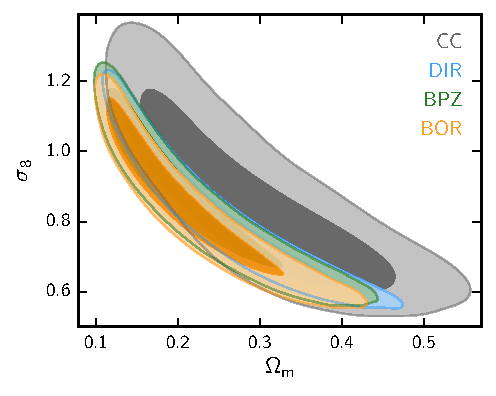
\includegraphics[width=0.5\textwidth]{kids450_fig7.pdf}

KiDS-450 measurements of the amplitude of large-scale clustering, compared to the standard Planck cosmology prediction. 68- and 95-percent contours are shown, both for the DIR and CC photometric redshift calibration methods.  {\bf UPDATE PLOT}

\bigskip

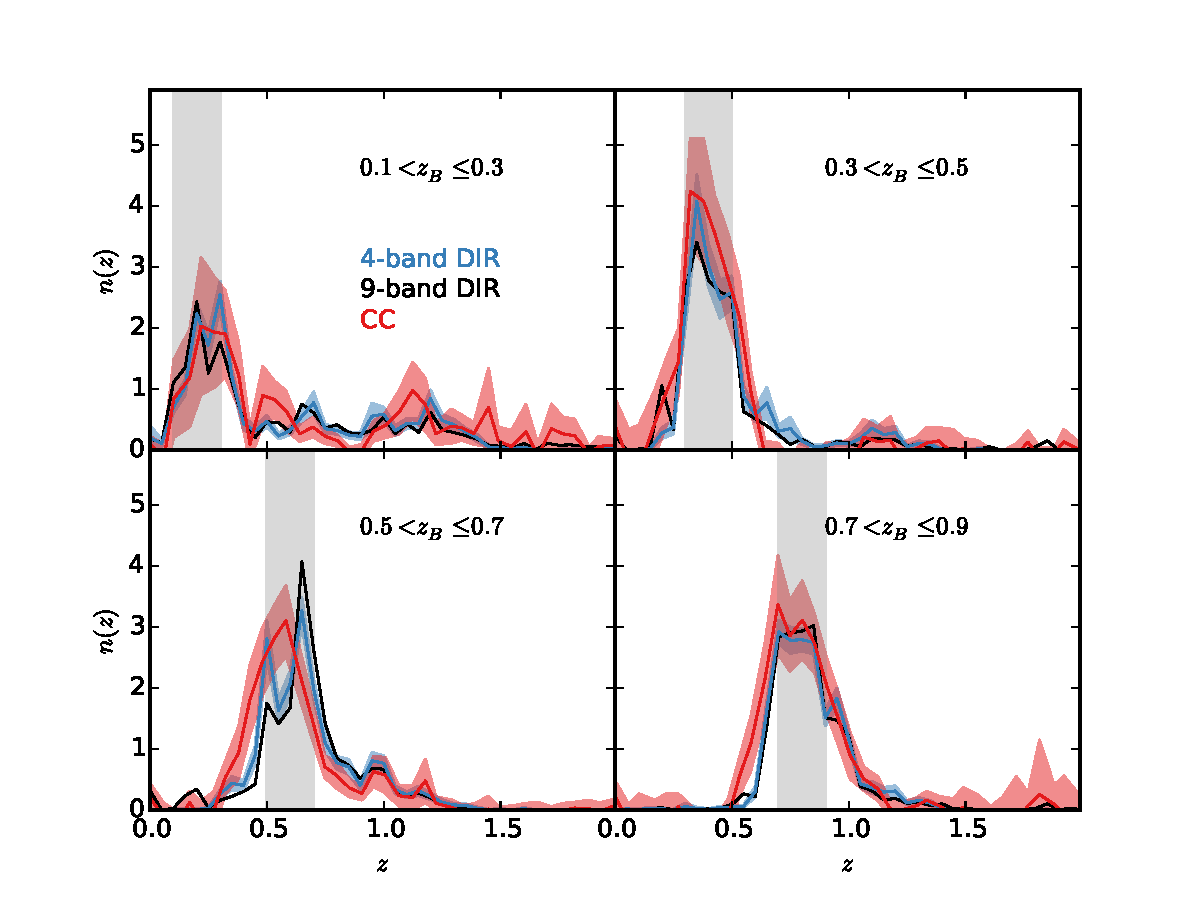
\includegraphics[width=0.5\textwidth]{Nz_comp_zall_4vs9vsCC.pdf}

Effect of including VISTA ZYJHK bands in the KiDS DIR photometric redshifts, and comparison with the CC distributions.

\bigskip

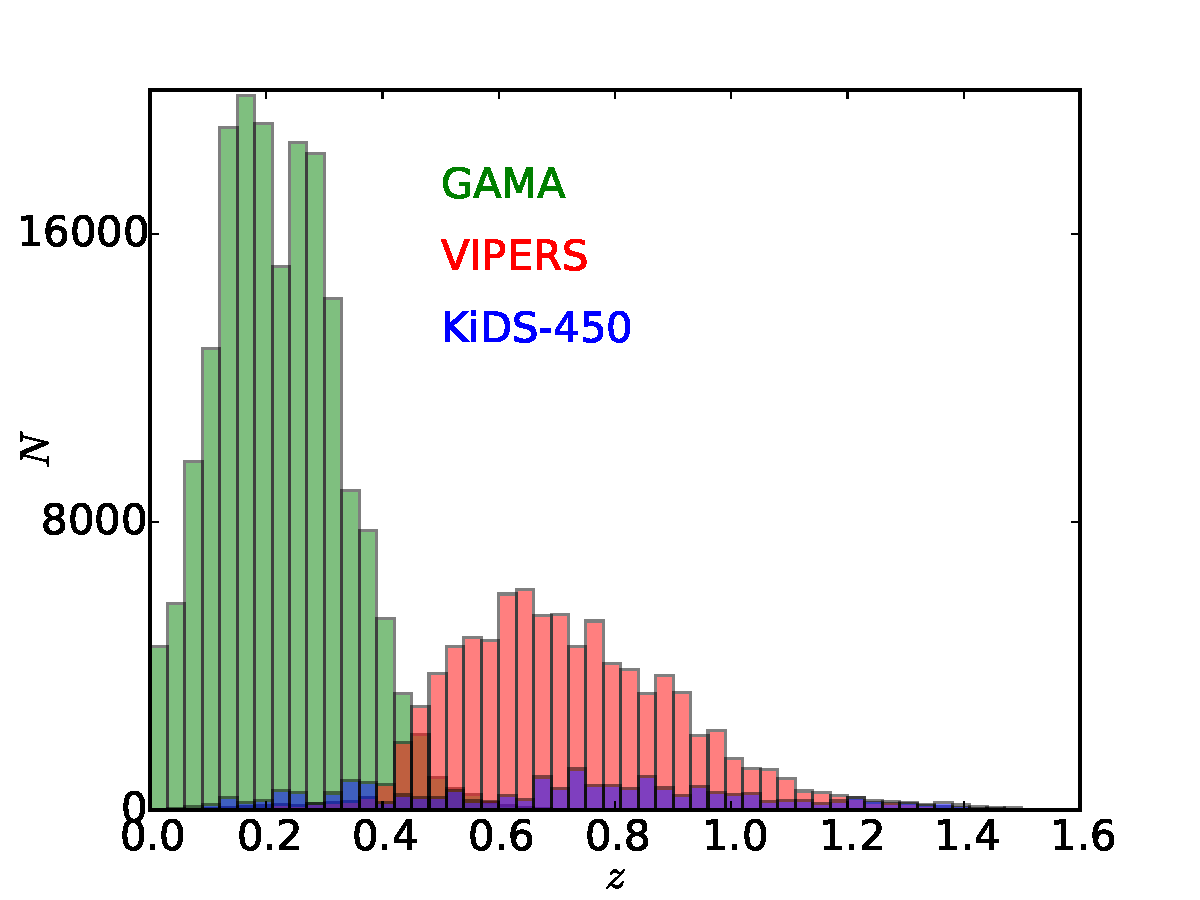
\includegraphics[width=0.5\textwidth]{ESO_prop_plot_zdist.pdf}

Compilation of available redshifts for CC calibration, together with those that were used in the published KiDS-450 so far. Incorporating VIKING data on the GAMA patches is in progress but will not help at redshifts beyond 0.5, for which we are proposing VIPERS coverage.

%\MakePicture{S8_Kilbinger.pdf}{width=0.6\hsize}
%\MakeCaption{Fig.~1: $S_8$ measurements}

%\MakePicture{Nz_comp_zall.pdf}{width=0.6\hsize,angle=0}
%\MakeCaption{Fig.~2: Redshift distributions}

\section*{8. Justification of requested time, lunar phase etc. (taken from DDT)}

WhyLunarPhase: 

No restrictions on the lunar phase for these near-infrared observations.

WhyNights:

We have requested the number of hours required to observe a single VISTA `tile' over each of the DEEP2 fields, using the same observation strategy as is  implemented in VIKING. Total exposure times per filter in VIKING are:

\vspace{0.5cm}
\begin{tabular}{rr}
filter & exp. time [s]\\
\hline
$Z$ & 480\\
$Y$ & 400\\
$J$ & 400\\
$H$ & 300\\
$Ks$ & 480\\
\hline
total & 2060\\
\end{tabular}

\vspace{0.5cm}
In order to attain these exposure times over a uniform area requires a six-step dither strategy that results in the majority of the area being covered by two dithers. Hence the required time on the telescope is three times as large, 6180s. With overheads we expect to be able to observe each field in 2h resulting in a total time request of 4h for our program.


\end{document}






This proposal concerns testing the standard LambdaCDM model of cosmology using tomographic weak lensing, specifically using the ESO public survey KiDS. Weak lensing measures the clustering of matter, irrespective of whether it is baryonic or not. Combined with redshift information of the lensed galaxies, such data can also constrain the growth rate of large-scale structure, a key cosmology observable. Currently, the most stringent measurements are those from KiDS (H++17), based on 450 square degrees of imaging data from the VST. More results are expected in the coming year from competing surveys (DES and HSC) as well as further KiDS data.

Intriguingly, the KiDS-450 result is in tension with the best-fit cosmology parameters from the CMB (Planck 2015): matter appears to be less clustered than this standard LCDM model predicts. A careful analysis of the potential sources of systematic error shows that this is dominated by the photometric redshifts which are used to assign galaxies to tomographic bins.

* little table with breakdown of errors on S8? shear (stat); shear (sys); nz (stat, DIR and CC), nz(sys,DIR and CC) ?

We have two independent methods for measuring n(z), which agree within errors. The next step is to improve their accuracy and precision.
DIR is a direct calibration of the mapping from colour space to redshifs, using spectroscopic redshifts as training. It requires spectroscopic data that cover the full *magnitude range* of the KiDS data.

CC uses clustering correlation with redshift slices. It requires a spectroscopic survey that spans the full *redshift range* of the KiDS galaxies. Currently we only have such data over 1.5 square degrees. Increasing the area by a factor of ten is required to reduce the statistical error to the same level as DIR and make it a subdominant part of the overall error budget of the cosmological analysis. *Banana plot to show this*

For the KiDS-450 analysis we used optical data only; we are in the process of adding in the five near-IR bands ZYJKH from the VIKING survey, which requires VISTA images on spectroscopic redshift calibration fields. In December we obtained DDT observations of two DEEP2 fields with VISTA, and we show preliminary results below. This experiment demonstrates the improvement that can be gained by moving from four to nine photometric bands. Currently this calibration is limited by cosmic variance, and we request two more deep fields here.

The KiDS footprint does not overlap with suitable spectroscopic surveys. Rather than embarking on a massive spectroscopy campaign on KiDS fields, we have therefore observed deep spectroscopic survey fields with KiDS-like VST imaging to establish this calibration. We now wish to extend this strategy to the five near-IR bands as well.

For CC


quantify how much area needed. Used 1.5 sqdeg for K450. comparing z=0.7 to 1.5 CC is 3.5x more noisy than DIR.
CC error needs to come down so complementary analysis has proper value
argue VIPERS OK even though redshift-selected; can combine with low-z info from GAMA.


